\documentclass[12pt]{article}
\usepackage[a4paper,margin=1in]{geometry}
\usepackage{hyperref}
\usepackage{enumitem}
\usepackage{tikz}
\hypersetup{
  colorlinks=true,
  linkcolor=blue,
  urlcolor=blue
}

\title{Understanding the Echo vs. Pressure Indexer Repository}
\author{Friendly Guide}
\date{\today}

\begin{document}
\maketitle

\begin{abstract}
This guide explains, step by step, what the repository does. It assumes no prior knowledge of coding. You will learn what problem the tool solves, how its parts cooperate, and how to run it on your own folder of comma-separated values (CSV) files. Simple diagrams and walk-through examples illustrate every major idea.
\end{abstract}

\section{The Big Picture}
Imagine you have many folders filled with CSV files recorded by a medical device. Each folder may contain one special file called \texttt{pressure.csv} plus several ``echo'' CSV files. The repository builds a compact report that:
\begin{enumerate}[label=\arabic*.]
  \item Lists every folder that holds CSV data.
  \item Pairs each echo file with the matching \texttt{pressure.csv} file (if it exists).
  \item Summarises sizes and table shapes so you can quickly spot empty or suspicious files.
  \item Records any problems, such as missing \texttt{pressure.csv} files, in an error log.
\end{enumerate}
All of this happens automatically when you point the tool at the top-level folder (called the \textbf{address}).

\section{Meet the Main Characters}
The repository is a small Python package living in the \texttt{src/indexer} directory. The most important files are:
\begin{description}[style=multiline,labelwidth=3.5cm]
  \item[\texttt{main.py}] Provides the command-line interface (CLI). It reads your input, checks the folders, and coordinates the scan.
  \item[\texttt{scanner.py}] Walks through the folders, gathers statistics about the CSV files, and records any errors.
  \item[\texttt{io\_helpers.py}] Supplies utility functions for reading CSV sizes, writing JSON/CSV outputs, and creating folders safely.
  \item[\texttt{models.py}] Defines a simple data container, \texttt{EchoEntry}, that pairs echo files with \texttt{pressure.csv}.
\end{description}
These files work together like stations on an assembly line: the CLI receives your request, the scanner analyses the data, and the helpers save the results.

\section{Step-by-Step Tour}
\subsection{Starting the Scan}
When you run the command-line tool, \texttt{main.py} does the following:
\begin{enumerate}
  \item Reads the \texttt{--address} you supplied and confirms the folder exists.
  \item Creates an output directory (defaults to \texttt{artifacts}).
  \item Calls \texttt{scan\_address} from \texttt{scanner.py} to explore the data.
\end{enumerate}
If the folder cannot be reached (for example, the path is mistyped), the program stops immediately and explains what went wrong.

\subsection{Finding Dataset Folders}
The function \texttt{find\_all\_dataset\_folders} examines the address and its subfolders. A folder qualifies as a \textbf{dataset folder} if it contains at least one CSV file. Two key rules apply:
\begin{itemize}
  \item If you point to a file, the tool switches to that file's parent folder.
  \item If multiple folders share the same name, the tool renames duplicates with \#2, \#3, and so on, to keep them unique.
\end{itemize}

\subsection{Inspecting Each Folder}
For every dataset folder, \texttt{scan\_dataset\_folder} gathers details:
\begin{enumerate}
  \item It searches for \texttt{pressure.csv} (case-insensitive) and remembers its size and row/column counts.
  \item It treats every other CSV file as an echo file. For each echo, it records:
  \begin{itemize}
    \item File name.
    \item Number of data rows (ignoring the header).
    \item Number of columns.
    \item File size in bytes.
  \end{itemize}
  \item If \texttt{pressure.csv} is missing or an echo file is empty, the tool adds a helpful note.
\end{enumerate}
If a folder contains only \texttt{pressure.csv}, the tool still emits a summary row so you know the folder was checked.

\subsection{Producing the Outputs}
Once every folder has been scanned, the tool writes three files into the output directory:
\begin{description}[style=multiline,labelwidth=3.2cm]
  \item[\texttt{dataset\_index.json}] A machine- and human-readable map from folder names to pairs of echo and pressure files.
  \item[\texttt{summary.csv}] A table with one row per echo file (plus any ``pressure-only'' folders). The table lists shapes, file sizes, and notes.
  \item[\texttt{errors.log}] A plain-text file listing any serious issues, such as missing \texttt{pressure.csv} files or unreadable data.
\end{description}
All writing is handled by \texttt{io\_helpers.py}, which creates temporary files first and then swaps them into place. This prevents half-written files if the process is interrupted.

\section{Hands-On Example}
Suppose your storage device contains the folders in Figure~\ref{fig:tree}. Each arrow points to the CSV files inside a dataset folder.

\begin{figure}[h]
\centering
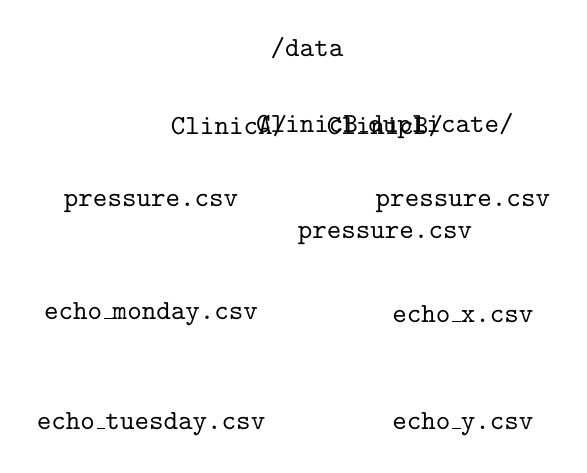
\begin{tikzpicture}[>=stealth, node distance=1.4cm]
  \node (root) {\texttt{/data}};
  \node[below left of=root] (a) {\texttt{ClinicA/}};
  \node[below right of=root] (b) {\texttt{ClinicB/}};
  \node[below left of=a] (a1) {\texttt{pressure.csv}};
  \node[below of=a1] (a2) {\texttt{echo\_monday.csv}};
  \node[below of=a2] (a3) {\texttt{echo\_tuesday.csv}};
  \node[below right of=b] (b1) {\texttt{pressure.csv}};
  \node[below of=b1] (b2) {\texttt{echo\_x.csv}};
  \node[below of=b2] (b3) {\texttt{echo\_y.csv}};
  \node[below right of=root] (c) {\texttt{ClinicB\_duplicate/}};
  \node[below of=c] (c1) {\texttt{pressure.csv}};
\end{tikzpicture}
\caption{Sample folder layout inspected by the indexer.}
\label{fig:tree}
\end{figure}

Running the tool with
\begin{verbatim}
python -m indexer.main --address /data --outdir artifacts
\end{verbatim}
produces:
\begin{itemize}
  \item \texttt{dataset\_index.json}
\begin{verbatim}
{
  "ClinicA": [
    {"echo": "echo_monday.csv", "press": "pressure.csv"},
    {"echo": "echo_tuesday.csv", "press": "pressure.csv"}
  ],
  "ClinicB": [
    {"echo": "echo_x.csv", "press": "pressure.csv"},
    {"echo": "echo_y.csv", "press": "pressure.csv"}
  ],
  "ClinicB_duplicate": [
    {"echo": null, "press": "pressure.csv"}
  ]
}
\end{verbatim}
  The final entry shows a folder that only contained \texttt{pressure.csv}. The tool still tells you it was seen.

  \item \texttt{summary.csv}
\begin{verbatim}
folder_path,echo_file,echo_rows,echo_cols,echo_size_bytes,pressure_file,pressure_rows,pressure_cols,pressure_size_bytes,note
/data/ClinicA,echo_monday.csv,123,10,2048,pressure.csv,456,12,4096,
/data/ClinicA,echo_tuesday.csv,117,10,1980,pressure.csv,456,12,4096,
/data/ClinicB,echo_x.csv,98,11,1820,pressure.csv,512,14,4200,
/data/ClinicB,echo_y.csv,101,11,1850,pressure.csv,512,14,4200,
/data/ClinicB_duplicate,,,,,pressure.csv,512,14,4200,only_pressure_csv
\end{verbatim}
  Empty cells in the ``echo'' columns show that no echo file was present in the duplicate folder.

  \item \texttt{errors.log}
\begin{verbatim}
pressure.csv not found in /data/ClinicB_duplicate
\end{verbatim}
  This reminds you to double-check the folder.
\end{itemize}

\section{How the Tool Reads CSV Files}
The helper function \texttt{csv\_shape} opens each file carefully:
\begin{enumerate}
  \item It tries to read using standard UTF-8 text encoding.
  \item If characters cannot be decoded, it retries with Latin-1 encoding.
  \item It counts how many non-empty rows follow the header line, ensuring that rows with only commas or blank spaces do not inflate the counts.
\end{enumerate}
If all attempts fail, it logs the issue and returns \texttt{(0, 0)} so the summary highlights the problem.

\section{Command Summary for Daily Use}
To use the repository on a new computer:
\begin{enumerate}
  \item Install dependencies: \texttt{pip install -e .}
  \item Run the CLI (replace the example path with your data location):
\begin{verbatim}
dset-index --address "~/MyData" --outdir "~/MyData/artifacts"
\end{verbatim}
  \item Inspect the files inside the output directory.
\end{enumerate}

\section{Troubleshooting}
\begin{itemize}
  \item \textbf{``Address does not exist'' error:} Check for typos in the folder path. The program halts immediately to avoid scanning the wrong place.
  \item \textbf{Empty row counts:} Confirm that your CSV file has a header and at least one data row. The summary will show \texttt{0} rows if the file is empty or unreadable.
  \item \textbf{Permission warnings:} If a folder cannot be opened, the tool skips it and records the problem so you can adjust permissions.
\end{itemize}

\section{Key Takeaways}
\begin{itemize}
  \item You only need to provide the top-level folder (the address); the tool handles the rest.
  \item Outputs are designed for both humans and machines, making follow-up analysis simple.
  \item Robust error handling means you always know which folders were scanned and where issues occurred.
\end{itemize}

\end{document}
